\section{Generación de señalamiento paso a paso}

	Inicialmente, el RNA ejecuta el Algoritmo \ref{alg:graph_network} (ver Sección \ref{sec:grafos}) para detectar todos los \textit{netElements}, sus coordenadas iniciales y finales en la topología, y el sentido en el que fueron definidas. Al concluir el Algoritmo \ref{alg:graph_network}, el RNA ejecuta el Algoritmo \ref{alg:connectedness} (ver Sección \ref{sec:grafos}) para analizar la conexidad de la red. El resultado obtenido se muestra en el Código \ref{lst:EJ7_1}, donde se describen las coordenadas de cada \textit{netElement} y se confirma que la red es conexa.
	
	\begin{lstlisting}[language = {}, caption = Detección de \textit{netElements} por parte del RNA , label = {lst:EJ7_1}]
	###### Starting Railway Network Analyzer #####
	Reading .railML file
	Creating railML object
	Analyzing railML object
	Analyzing graph
	ne1 [-770, -30] [260, -30] >>
	ne31 [554, 480] [1190, 480] >>
	ne32 [554, 480] [1460, 957] >>
	ne40 [260, -30] [554, 480] >>
	ne41 [260, -30] [1040, -420] >>
	ne42 [1040, -420] [1730, -420] >>
	ne43 [1040, -420] [440, -420] <<
	The network is connected
	\end{lstlisting}
	
	Por ejemplo, el \textit{netElement} ne42 inicia en la coordenada (1040;-420) y finaliza en la coordenada (1730;-420). El símbolo $>>$ indica que ne1 se encuentra definido de izquierda a derecha, ya que la componente x de la coordenada final es mayor a la de la coordenada inicial, teniendo la misma componente y. Además, se puede comprobar que la lista obtenida en consistente con la Figura \ref{fig:EJ7_2}. Por ejemplo, ne1, ne40 y ne41 comparten la coordenada (260;-30), que coincide con la coordenada del cambio de vías Sw18.
	
	A continuación, el RNA detectará la infraestructura ferroviaria, las curvas peligrosas y los puntos medios de los netElements que el RNA considera demasiado largos. El análisis de la infraestructura se detalla en la Sección \ref{sec:bufferstop}, Sección \ref{sec:detectors}, Sección \ref{sec:platform} y Sección \ref{sec:crossing}, mientras que la detección de curvas y puntos medios se detalla en la Sección \ref{sec:tracks}. El RNA ejecuta el Algoritmo \ref{alg:switches_1}, Algoritmo \ref{alg:switches_2} y Algoritmo \ref{alg:switches_3} para confirmar la detección de cambios de vías simples, dobles y en tijeras. El resultado de este proceso se puede visualizar en el Código \ref{lst:EJ7_2}.
	
	\begin{lstlisting}[language = {}, caption = Detección de puntos críticos por parte del RNA , label = {lst:EJ7_2}]
	Analyzing infrastructure --> Infrastructure.RNA
	Detecting Danger --> Safe_points.RNA
	ne1 has a Middle point @ [-564.0, -30]
	ne1 has a Middle point @ [-358.0, -30]
	ne1 has a Middle point @ [-152.0, -30]
	ne1 has a Middle point @ [54.0, -30]
	ne31 has a Middle point @ [766.0, 480]
	ne31 has a Middle point @ [978.0, 480]
	ne32 has a Curve(2 lines) @ [[830, 957]]
	ne41 has a Curve(2 lines) @ [[650, -30]]
	ne42 has a Middle point @ [1270.0, -420]
	ne42 has a Middle point @ [1500.0, -420]
	ne43 has a Middle point @ [640.0, -420]
	ne43 has a Middle point @ [840.0, -420]
	\end{lstlisting}
	
	Esta información es exportada por el RNA, con mayor detalle, en el archivo Infrastructure.RNA (Código \ref{lst:EJ7_4}) que resume cada elemento ferroviario asociado a su respectivo \textit{netElement}.
	
	\begin{lstlisting}[language = {}, caption = Infrastructure.RNA, label = {lst:EJ7_4}]
Nodes: 7|Switches: 3|Signals: 0|Detectors: 0|Ends: 5|Barriers: 0
Node ne1:
	Track = track1
	Type = BufferStop -> ['bus1']
	Neighbours = 2 -> ['ne41', 'ne40']
	Switches -> Sw18
		ContinueCourse -> right -> ne41
		BranchCourse -> left -> ne40
Node ne31:
	Track = track2
	Type = BufferStop -> ['bus4']
	Neighbours = 2 -> ['ne40', 'ne32']
Node ne32:
	Track = track4
	Type = BufferStop -> ['bus35']
	Neighbours = 2 -> ['ne31', 'ne40']
Node ne40:
	Track = track3
	Neighbours = 4 -> ['ne1', 'ne31', 'ne32', 'ne41']
	Switches -> Sw14
		ContinueCourse -> left -> ne32
		BranchCourse -> right -> ne31
Node ne41:
	Track = track5
	Neighbours = 4 -> ['ne1', 'ne40', 'ne42', 'ne43']
Node ne42:
	Track = track6
	Type = BufferStop -> ['bus48']
	Neighbours = 2 -> ['ne41', 'ne43']
	Switches -> Sw19
		ContinueCourse -> left -> ne43
		BranchCourse -> right -> ne41
Node ne43:
	Track = track7
	Type = BufferStop -> ['bus47']
	Neighbours = 2 -> ['ne41', 'ne42']
	\end{lstlisting}
	
	La información de la infraestructura es utilizada por el RNA para detectar los puntos críticos de la red, es decir, las zonas donde es recomendable colocar una señal, según el sentido de circulación que se desee. El resultado es exportado al archivo SafePoints.RNA (Código \ref{lst:EJ7_5}). En el caso de que un mismo \textit{netElement} tenga más de un punto crítico para el mismo sentido, el RNA tomará el más cercano al elemento a proteger. El criterio de selección de puntos críticos se aplica para cada elemento ferroviario detectado, cada curva y cada cambio de vías y fue explicado en las secciones correspondientes ya mencionadas.
	
	\begin{lstlisting}[language = {}, caption = SafePoints.RNA, label = {lst:EJ7_5}]
ne1:
	Next: [[-564.0, -30], [-358.0, -30], [-152.0, -30], [54.0, -30]]
	Prev: [[-564.0, -30], [-358.0, -30], [-152.0, -30], [54.0, -30]]
ne31:
	Next: [[766.0, 480], [978.0, 480]]
	Prev: [[766.0, 480], [978.0, 480]]
ne32:
	Prev: [[930.0, 957]]
ne41:
	Next: [[550.0, -30]]
ne42:
	Next: [[1270.0, -420], [1500.0, -420]]
	Prev: [[1270.0, -420], [1500.0, -420]]
ne43:
	Next: [[640.0, -420], [840.0, -420]]
	Prev: [[640.0, -420], [840.0, -420]]
	\end{lstlisting}	
	
	Una vez que el RNA detectó cada punto crítico de la red ferroviaria, procede a generar el señalamiento. El orden en que se procesan los elementos ferroviarios no impacta en el resultado final, pero para poder describirlo de forma ordenada se iniciará generando el señalamiento para proteger los finales de vías, las junturas entre rieles, las plataformas (explicado en la Sección \ref{sec:sig_platform}), los cruces de vía (explicado en la Sección \ref{sec:sig_levelcrossing}) y los cambios de vías (explicado en la Sección \ref{sec:signal_switches}). Luego se procederá a mostrar el señalamiento completo antes y después de la simplificación de señales (explicado en la Sección \ref{sec:simplificacion}). 
	
	Tal cómo se explicó en la Sección \ref{sec:sig_border}, el RNA aplica el Algoritmo \ref{alg:lineBorder} y el Algoritmo \ref{alg:bufferStop} para generar las señales para proteger los finales de vías relativos y absolutos. Estas señales son ilustradas en la Figura \ref{fig:EJ7_3}.
	
	\begin{figure}[H]
		\centering
		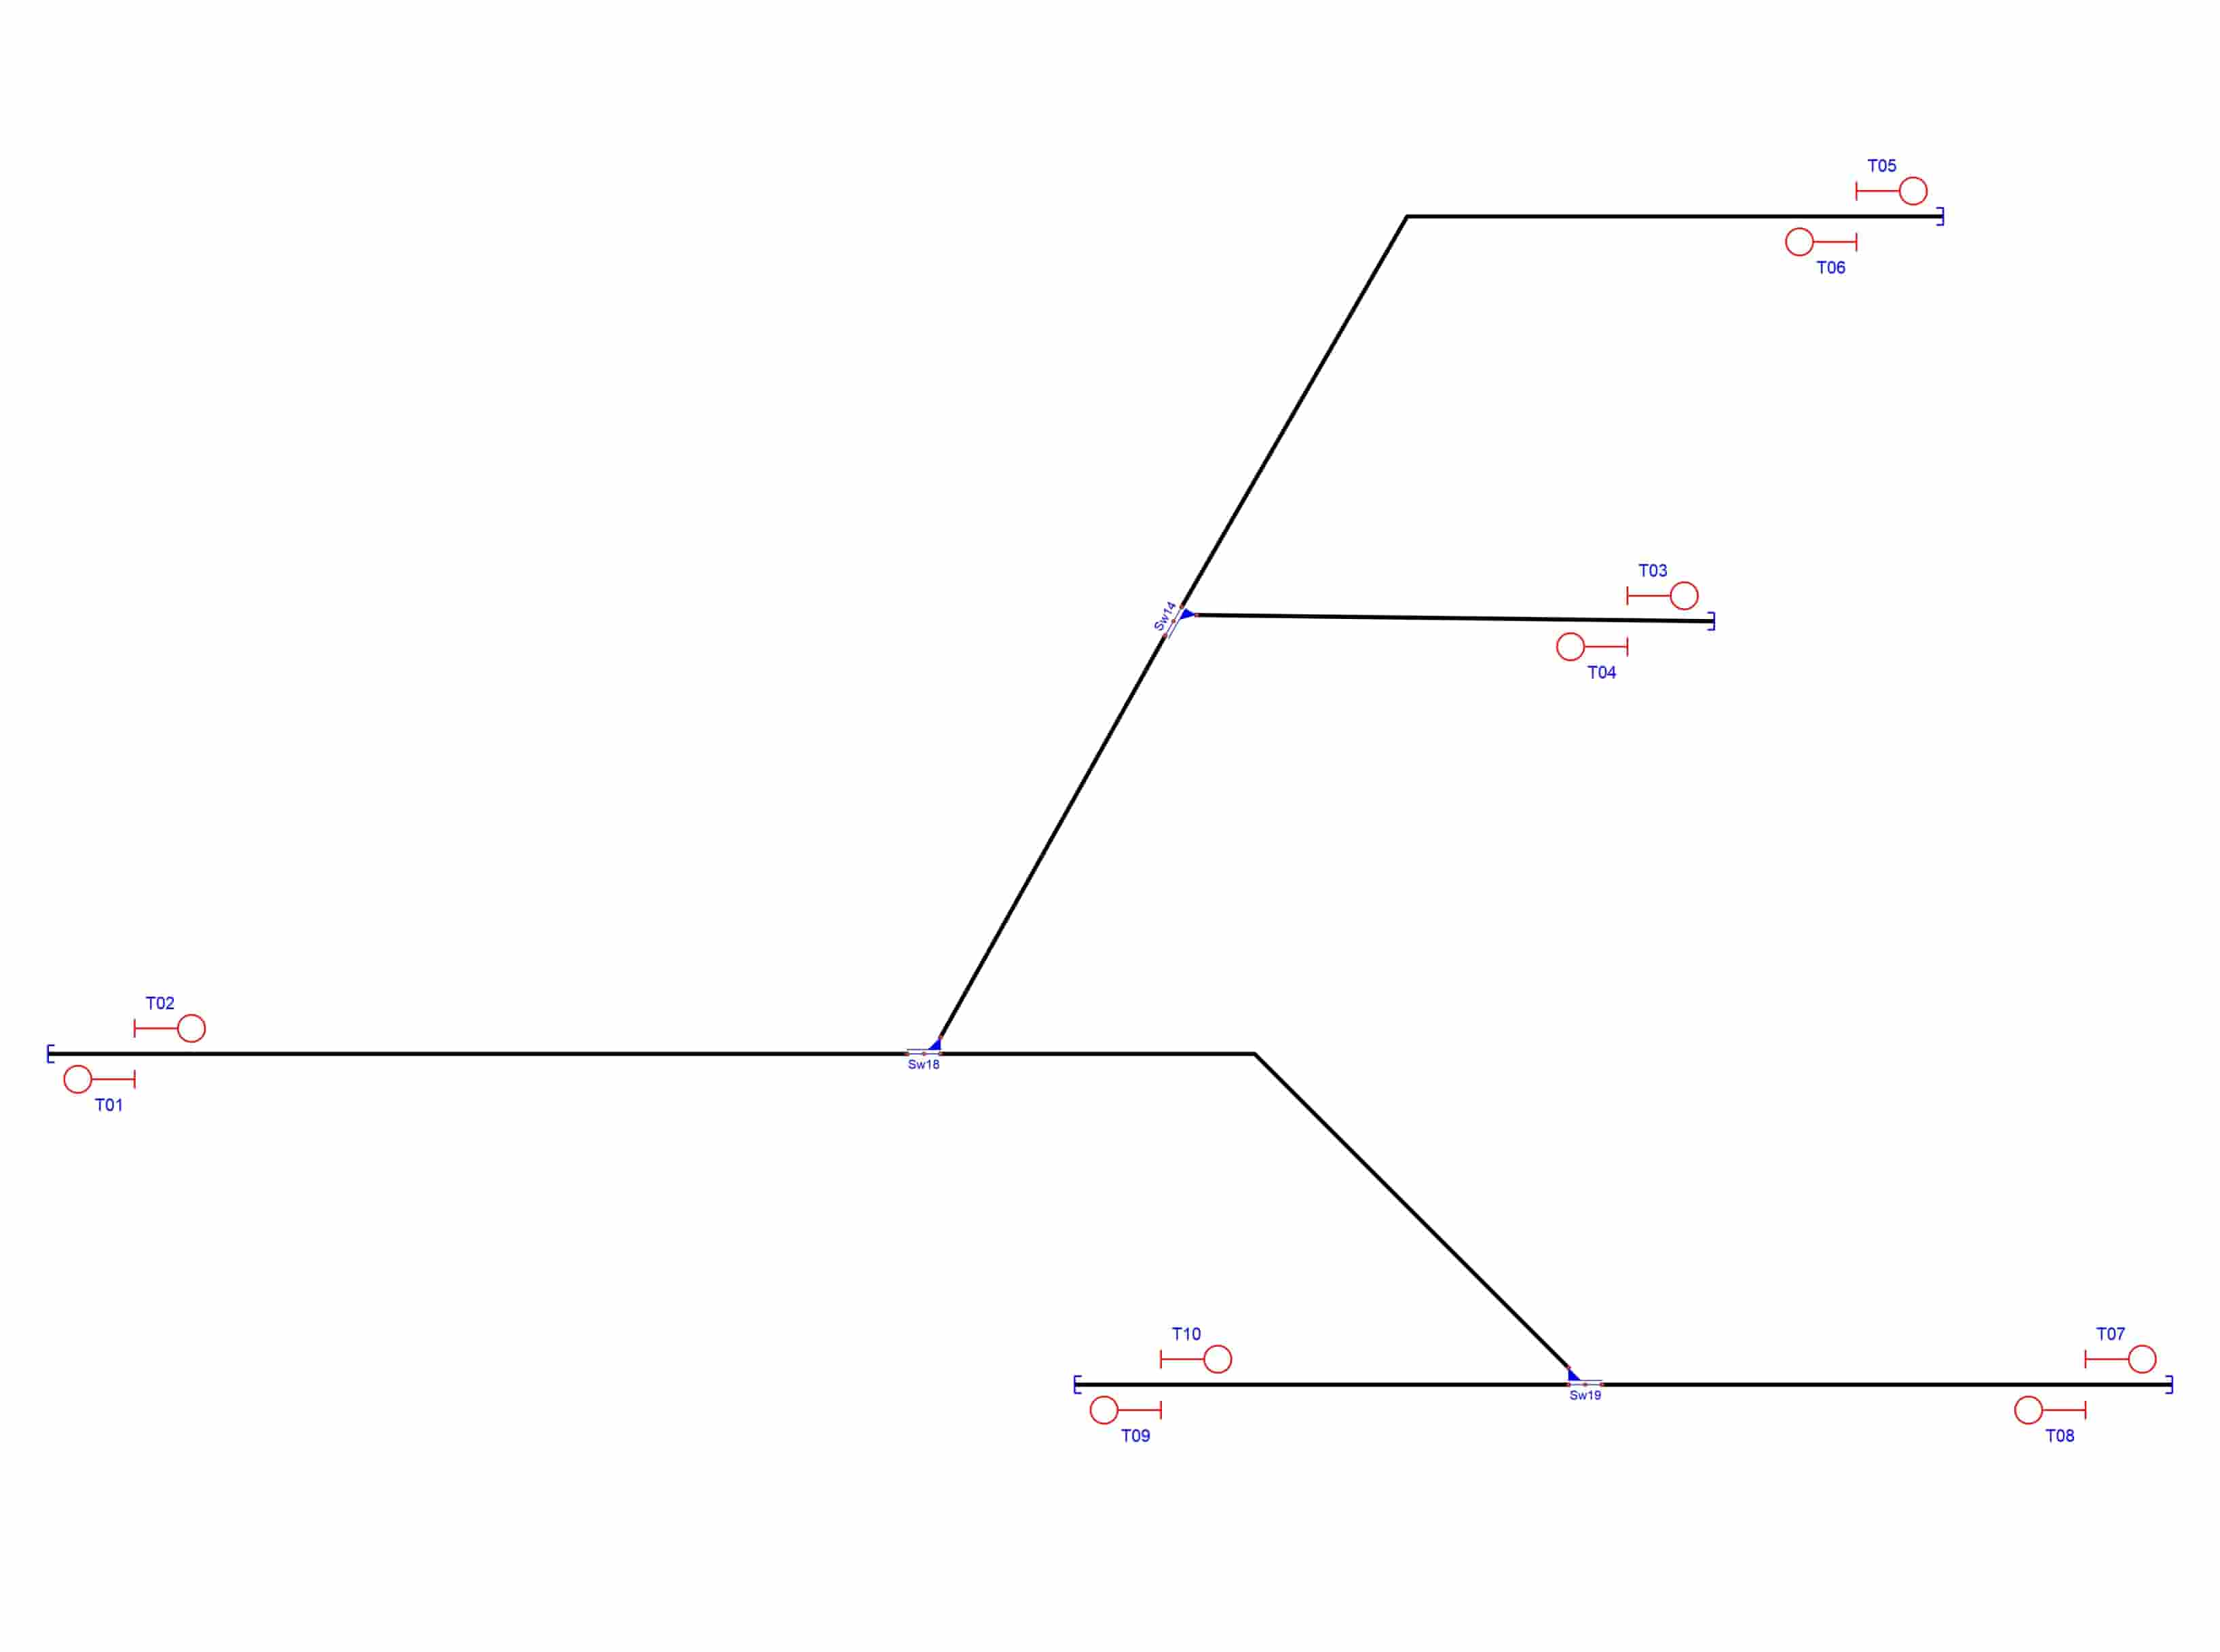
\includegraphics[width=1\textwidth]{resultados-obtenidos/ejemplo7/images/7_step1.png}
		\centering\caption{Señalamiento generado por el RNA para proteger el fin de vía.}
		\label{fig:EJ7_3}
	\end{figure}
	
	Los finales de vías absolutos son protegidos por las señales de parada T01, T03, T05, T07 y T09; y las señales de partida son T02, T04, T06, T08 y T10. No existen finales de vías relativos que proteger, por lo que el RNA asigno señalamiento para ese fin. Al tampoco existir junturas que proteger, la Figura \ref{fig:EJ7_4} no presenta cambios.
	
	\begin{figure}[H]
		\centering
		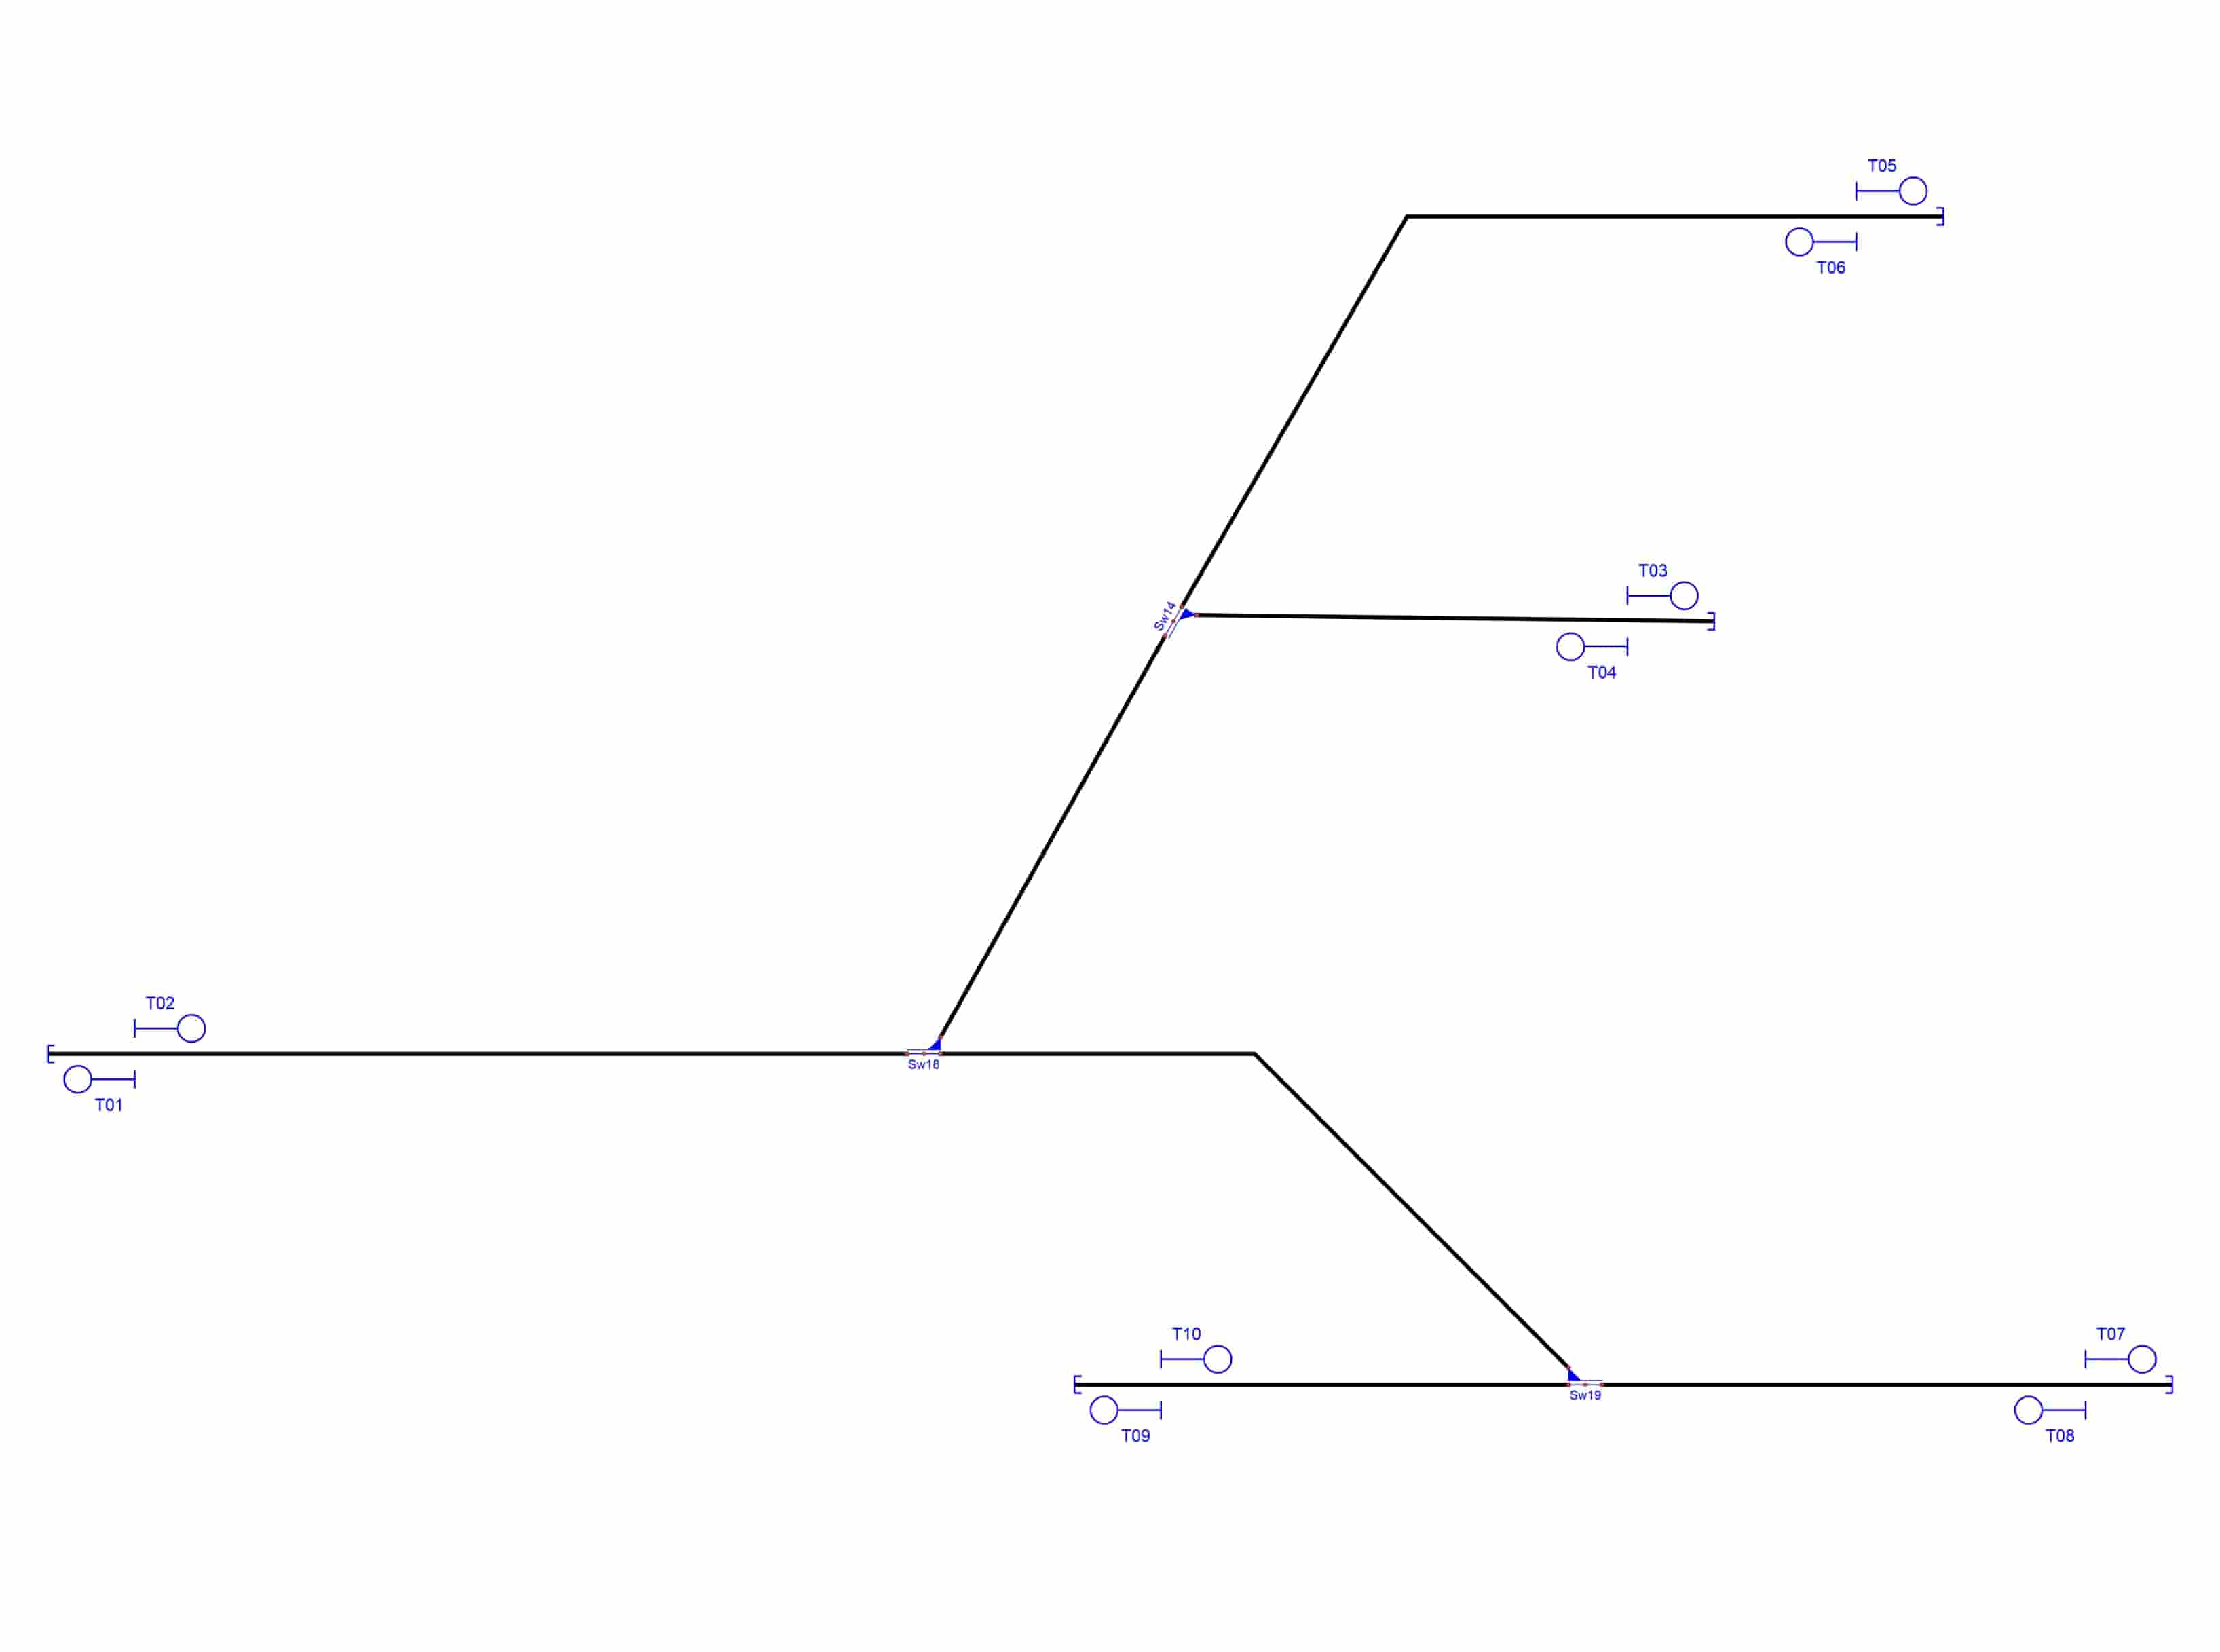
\includegraphics[width=1\textwidth]{resultados-obtenidos/ejemplo7/images/7_step2.png}
		\centering\caption{Señalamiento generado por el RNA para proteger las junturas.}
		\label{fig:EJ7_4}
	\end{figure}
	
	Al generar el señalamiento para proteger la infraestructura, tal como se explicó en la Sección \ref{sec:horizontal}, el Algoritmo \ref{alg:horizontal} simplificará las señales entre dos elementos ferroviarios si no existe espacio suficiente entre ellos. Al no existir plataformas o cruces de vías el señalamiento que se ilustra en la Figura \ref{fig:EJ7_5} no presenta cambios.
	
	\begin{figure}[H]
		\centering
		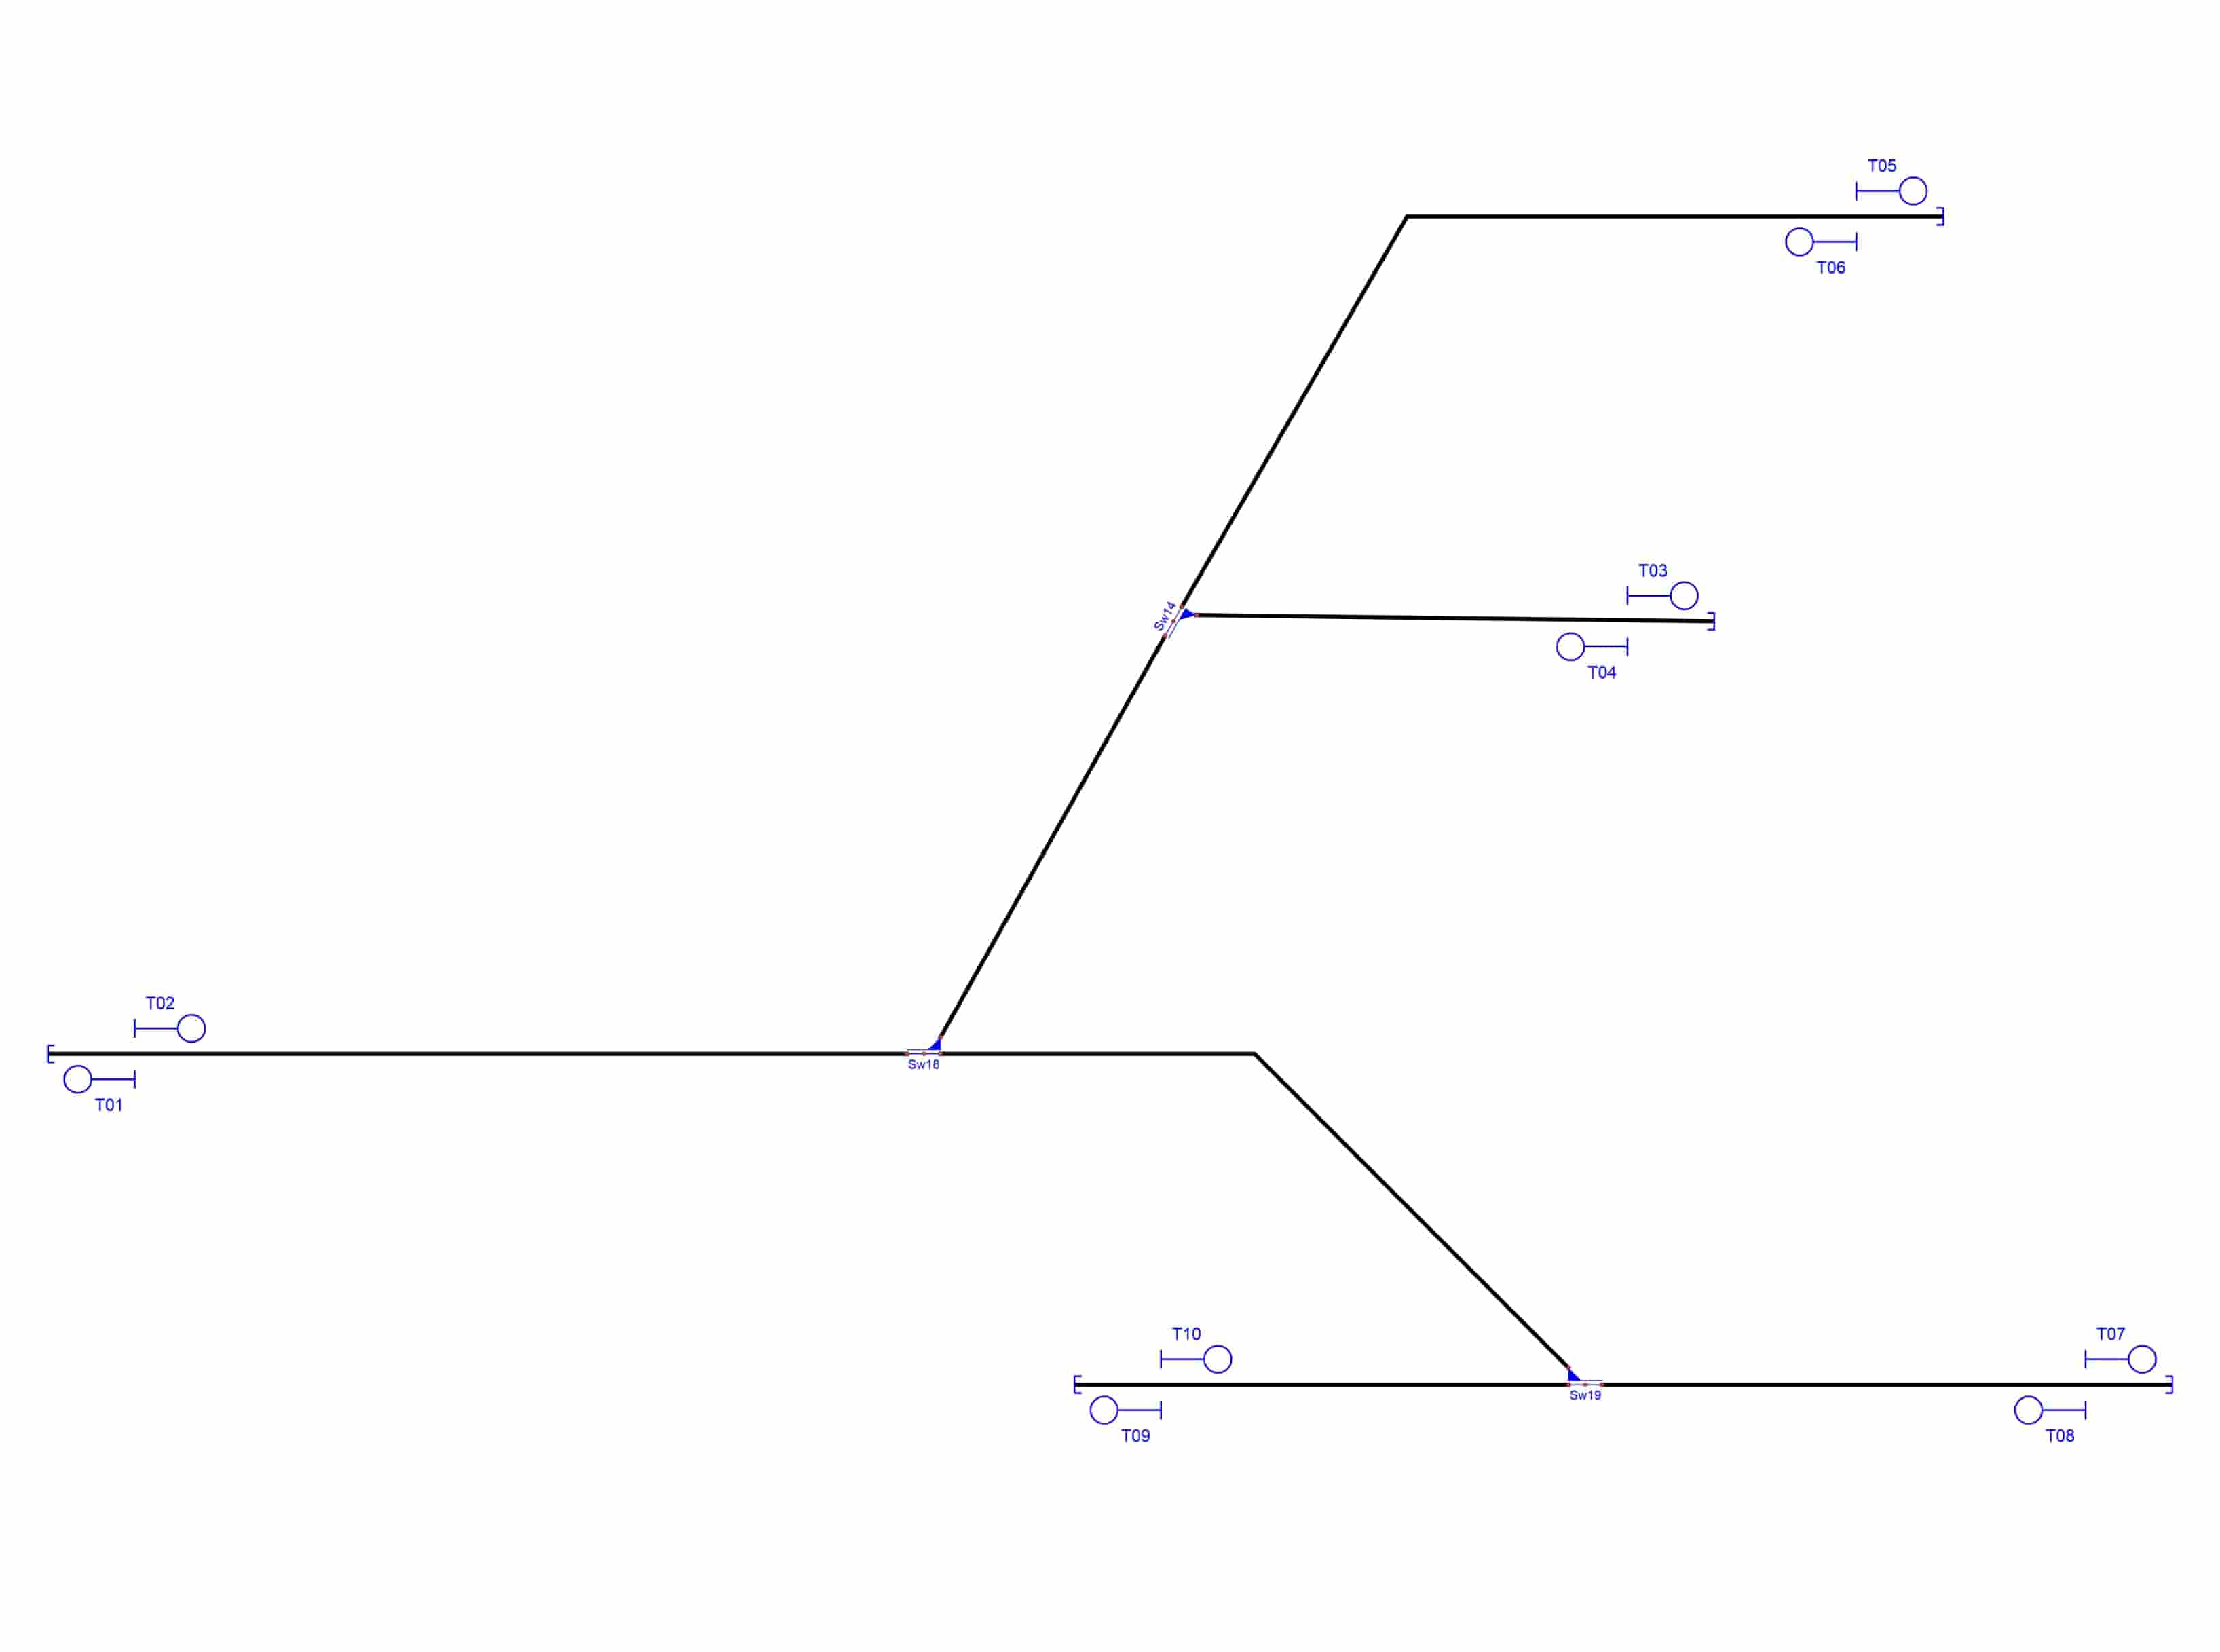
\includegraphics[width=1\textwidth]{resultados-obtenidos/ejemplo7/images/7_step3.png}
		\centering\caption{Señalamiento generado por el RNA para proteger plataformas y cruces de vía.}
		\label{fig:EJ7_5}
	\end{figure}
	
	Al aplicar el Algoritmo \ref{alg:SW} de generación de señalamiento para cambios de vías, tal como fue explicado en la Sección \label{sec:signal_switches}, el RNA genera las señales S14, C13 y H15 para proteger el cambio de vías Sw18; las señales C11, B12 y H16 para proteger el cambio de vías Sw14 y las señales S19, C17, B18 y H20 para proteger el cambio de vías Sw19. Las señales mencionadas se encuentran resaltadas en rojo en la Figura \ref{fig:EJ7_6}.
	
	\begin{figure}[H]
		\centering
		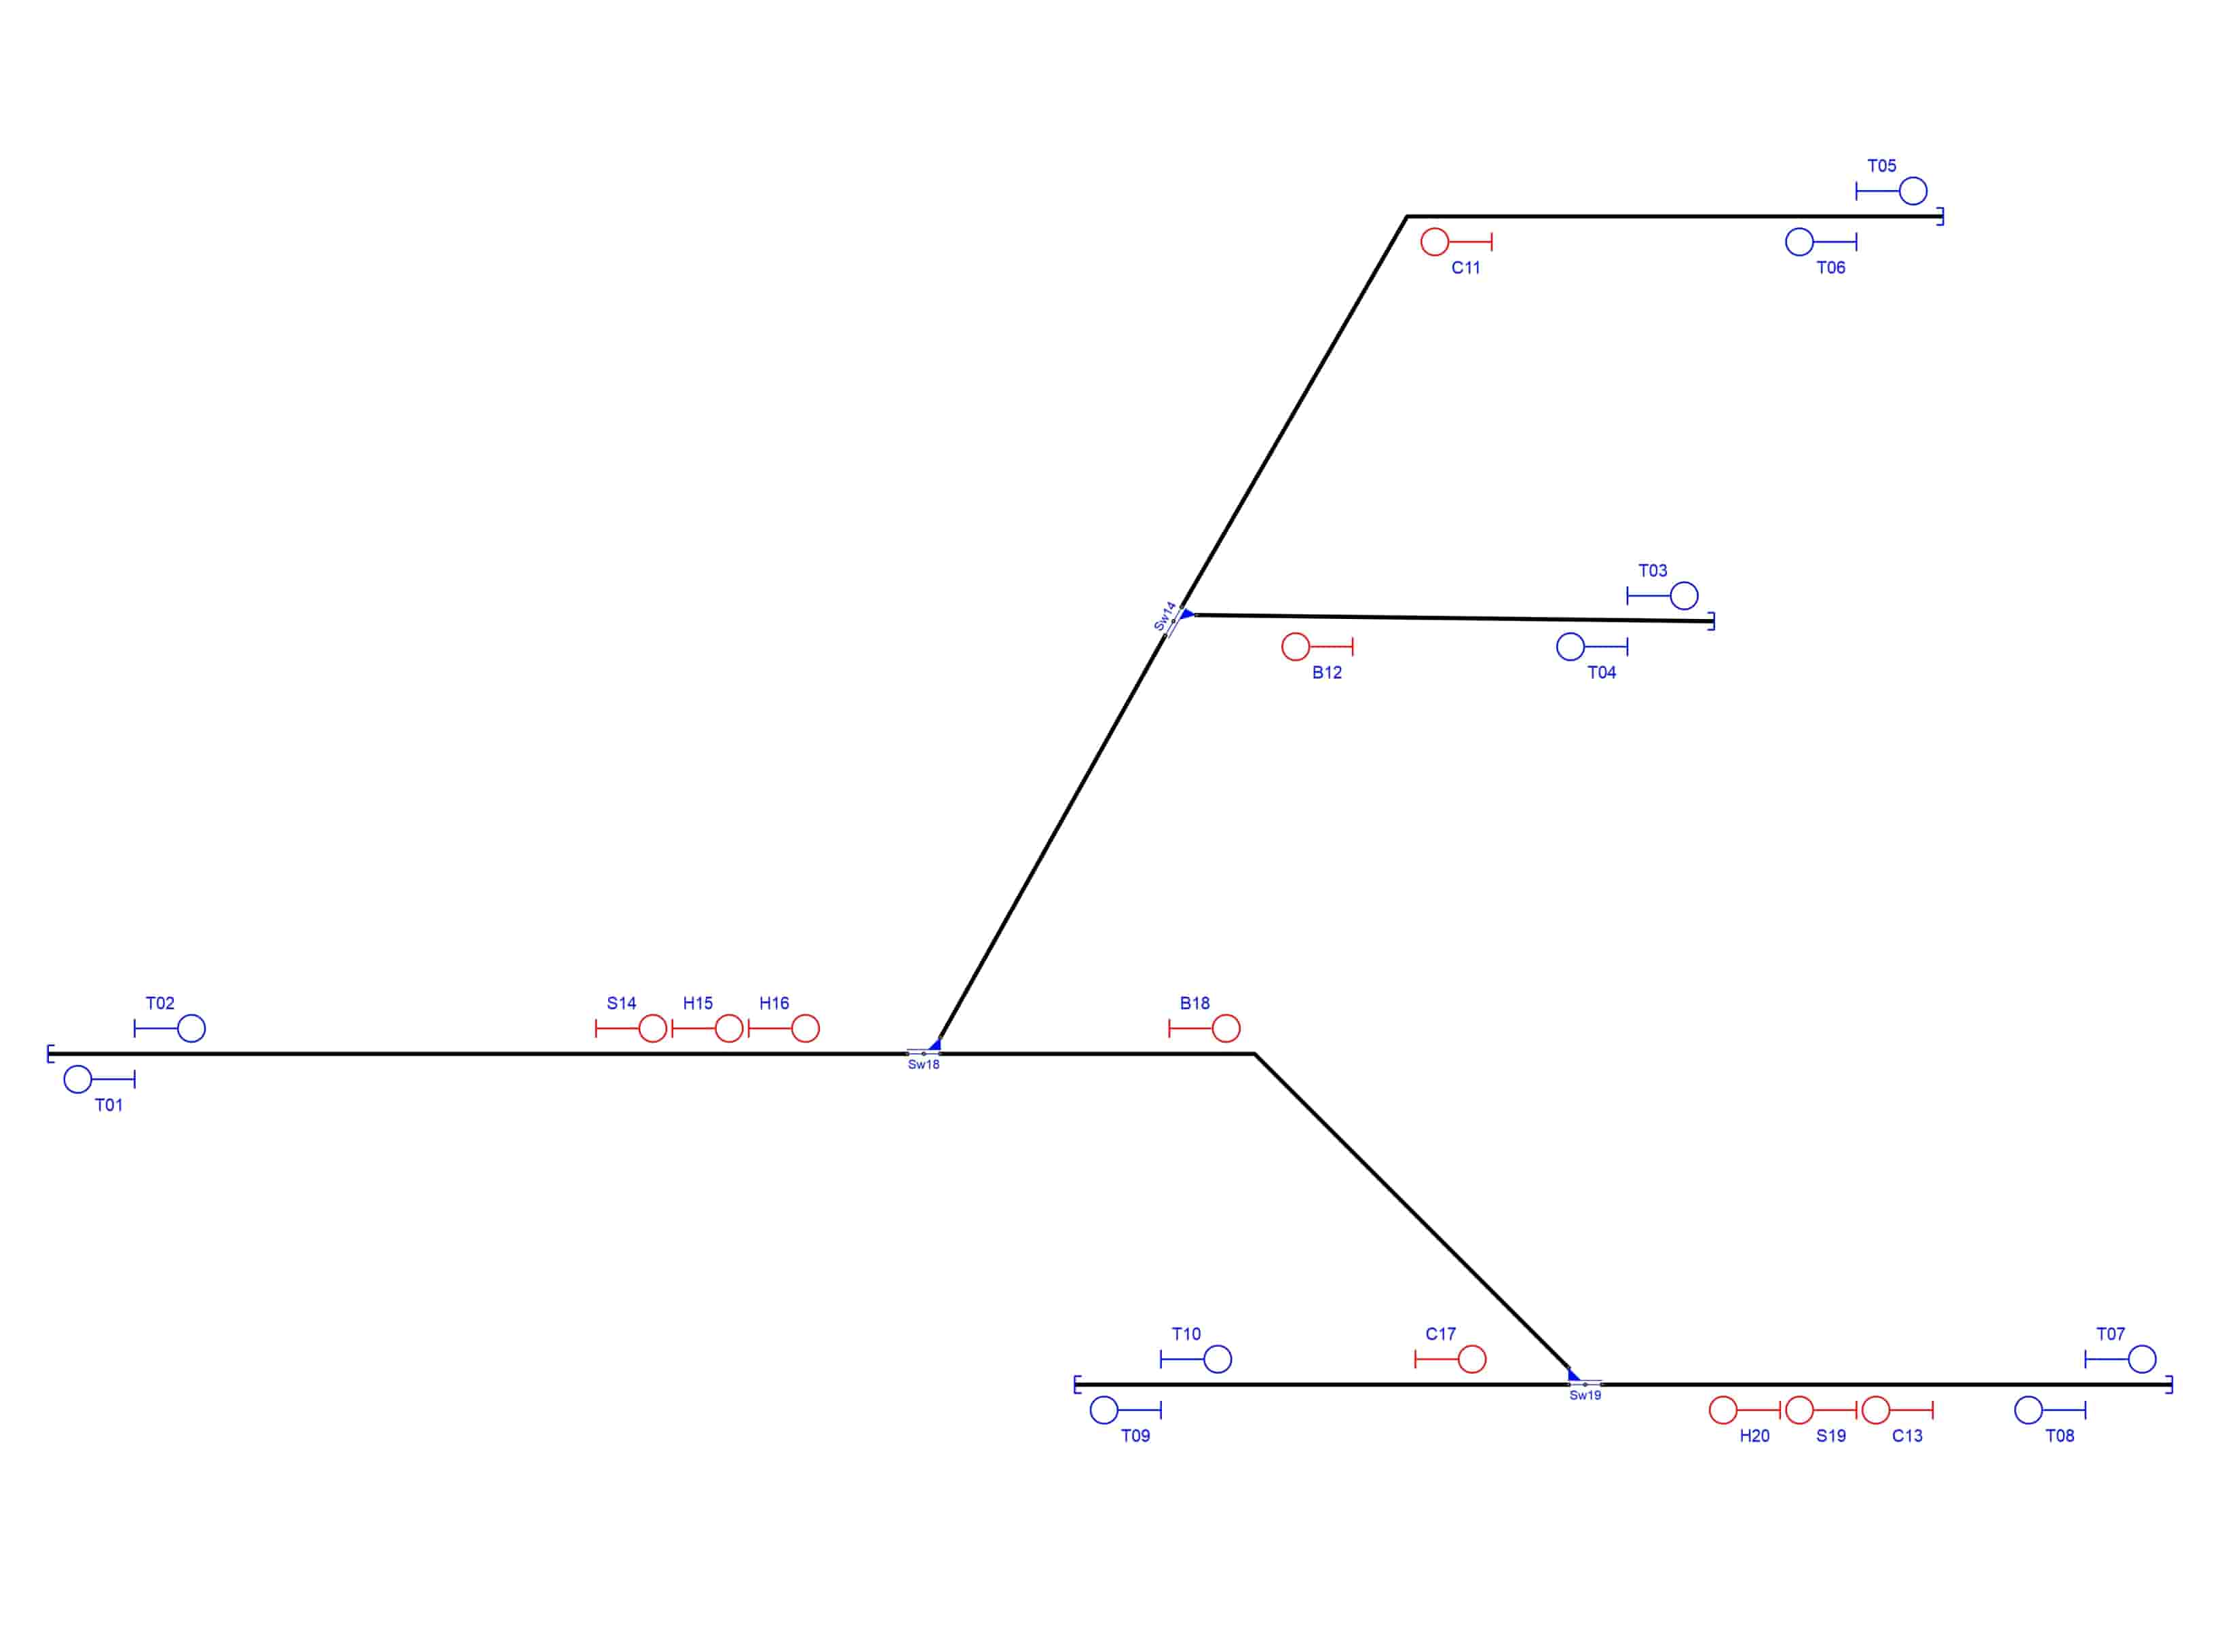
\includegraphics[width=1\textwidth]{resultados-obtenidos/ejemplo7/images/7_step4.png}
		\centering\caption{Señalamiento generado por el RNA para proteger los cambios de vías.}
		\label{fig:EJ7_6}
	\end{figure}
	
	Una vez obtenido todo el señalamiento, el RNA procede a simplificar las señales redundantes, repetidas o cuyas funciones o ubicaciones se superponen entre sí. El proceso de simplificación de señales fue explicado en la Sección \ref{sec:simplificacion}. El Algoritmo \ref{alg:vertical} de herencia vertical fue aplicado en las señales B entre los cambios de vías Sw18 y Sw19, desplazando las señales hasta convertirlas en las señales B12 y B18 respectivamente. Análogamente, las señales C y S del \textit{netElement} se convirtieron en las señales H15 y C17 respectivamente.
	
	Las señales simplificadas al aplicar el Algoritmo \ref{alg:horizontal} de herencia horizontal son: C11, B12, H15, H16, C17, C13, S19 y H20. Las señales H15 y H16 fueron eliminadas por su cercanía con la señal S14, con la cual comparten dirección y sentido. Lo mismo ocurre entre las señales H20 y C13. En todos los casos, se aplicó el Algoritmo \ref{alg:horizontal}, diseñado para agrupar objetos cercanos como un único objeto, generando el señalamiento acorde a los elementos contenidos en cada extremo del nuevo elemento contenedor.
	
	Finalmente, las señales son simplificadas aplicando el Algoritmo \ref{alg:reduction} de eliminación por prioridad de señales. El resultado de este proceso es detallado en el Código \ref{lst:EJ7_3}.
	
	\begin{lstlisting}[language = {}, caption = Reducción de señalamiento por prioridad de señales, label = {lst:EJ7_3}]
	Reducing redundant signals
	T priority removing sig12 for sig04
	T priority removing sig11 for sig06
	T priority removing sig13 for sig08
	T priority removing sig19 for sig08
	T priority removing sig17 for sig10
	Same position removing sig15 for sig14
	Same position removing sig16 for sig14
	Same position removing sig20 for sig13
	\end{lstlisting}
	
	El resultado de la simplificación del señalamiento se ilustra en la Figura \ref{fig:EJ7_7}.
	
	\begin{figure}[H]
		\centering
		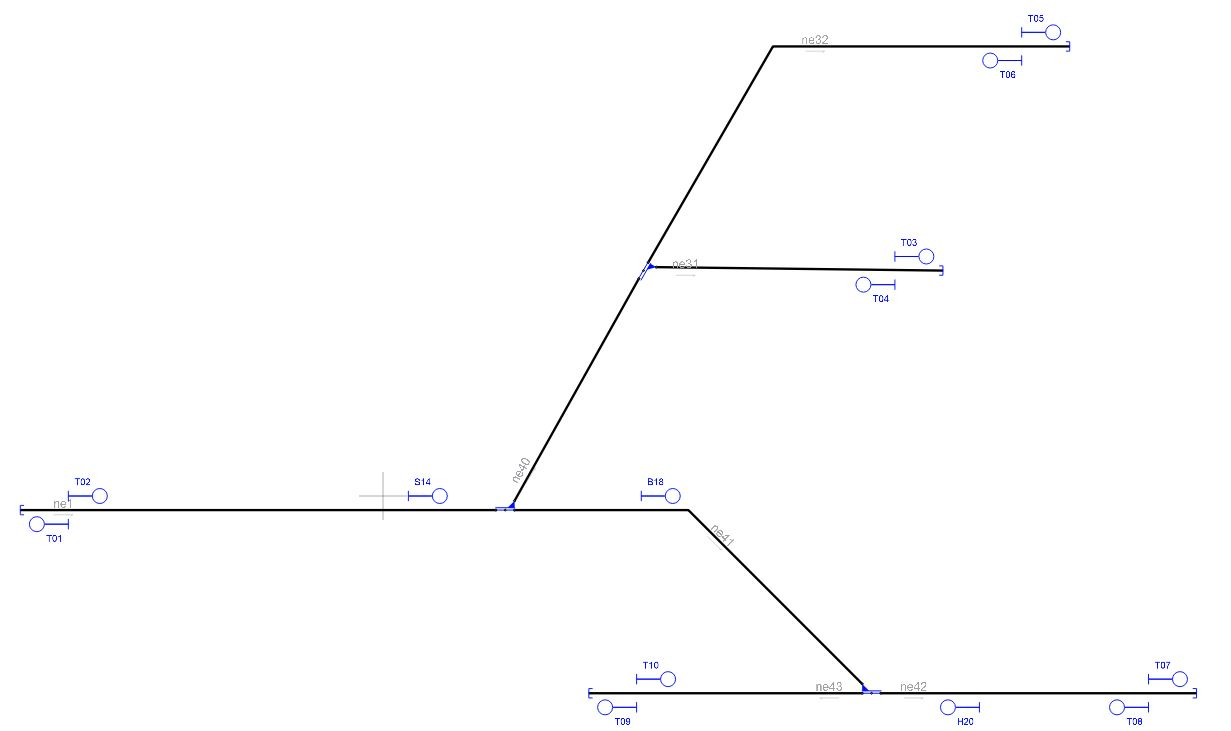
\includegraphics[width=1\textwidth]{resultados-obtenidos/ejemplo7/images/7_RNA.png}
		\centering\caption{Señalamiento generado y simplificado por el RNA.}
		\label{fig:EJ7_7}
	\end{figure}
	
	Además, toda la información del señalamiento generado es exportada por el RNA en el archivo Signalling.RNA (Código \ref{lst:EJ7_6}), que incluye información detallada de la posición, orientación, sentido, coordenada, nombre y tipo de señal.
	
	\begin{lstlisting}[language = {}, caption = Signalling.RNA, label = {lst:EJ7_6}]
sig01 [T01] <<:
	From: ne1 | To: bus1_left
	Type: Stop | Direction: reverse | AtTrack: right 
	Position: [-670, 30] | Coordinate: 0.0970
sig02 [T02] >>:
	From: ne1 | To: ne1_right
	Type: Stop | Direction: normal | AtTrack: left 
	Position: [-670, 30] | Coordinate: 0.0970
sig03 [T03] >>:
	From: ne31 | To: bus4_right
	Type: Stop | Direction: normal | AtTrack: left 
	Position: [1090, -480] | Coordinate: 0.8427
sig04 [T04] <<:
	From: ne31 | To: ne31_left
	Type: Stop | Direction: reverse | AtTrack: right 
	Position: [1090, -480] | Coordinate: 0.8427
sig05 [T05] >>:
	From: ne32 | To: bus35_right
	Type: Stop | Direction: normal | AtTrack: left 
	Position: [1360, -957] | Coordinate: 0.9153
sig06 [T06] <<:
	From: ne32 | To: ne32_left
	Type: Stop | Direction: reverse | AtTrack: right 
	Position: [1360, -957] | Coordinate: 0.9153
sig07 [T07] >>:
	From: ne42 | To: bus48_right
	Type: Stop | Direction: normal | AtTrack: left 
	Position: [1630, 420] | Coordinate: 0.8550
sig08 [T08] <<:
	From: ne42 | To: ne42_left
	Type: Stop | Direction: reverse | AtTrack: right 
	Position: [1630, 420] | Coordinate: 0.8550
sig09 [T09] <<:
	From: ne43 | To: bus47_left
	Type: Stop | Direction: normal | AtTrack: left 
	Position: [540, 420] | Coordinate: 0.1666
sig10 [T10] >>:
	From: ne43 | To: ne43_right
	Type: Stop | Direction: reverse | AtTrack: right 
	Position: [540, 420] | Coordinate: 0.1666
sig14 [S14] >>:
	From: ne1 | To: ne1_right
	Type: Circulation | Direction: normal | AtTrack: left 
	Position: [54.0, 30] | Coordinate: 0.8
sig18 [B18] >>:
	From: ne41 | To: ne41_right
	Type: Manouver | Direction: normal | AtTrack: left 
	Position: [550.0, 30] | Coordinate: 0.8937
sig20 [H20] <<:
	From: ne42 | To: ne42_left
	Type: Manouver | Direction: reverse | AtTrack: right 
	Position: [1270.0, 420] | Coordinate: 0.3333
	\end{lstlisting}
	
	Al finalizar la generación del señalamiento, el RNA ejecuta el Algoritmo \ref{alg:routes}, explicado en la Sección \ref{sec:rutas}, para detectar todas las posibles rutas admitidas por la red para crear la tabla de enclavamientos. La cuál puede ser visualizada en el archivo Routes.RNA (Código \ref{lst:EJ7_7}). La misma detalla las señales de inicio y final, los \textit{netElements} abarcados por la ruta y cualquier infraestructura involucrada, incluyendo el estado que deben tener para que la ruta sea activada.
	
	\begin{lstlisting}[language = {}, caption = Routes.RNA, label = {lst:EJ7_7}]
route_1 [sig02 >> sig14]:
	Path: ['ne1']
	Switches: ['Sw18']
route_2 [sig04 << sig01]:
	Path: ['ne31', 'ne40', 'ne1']
	Switches: ['Sw14', 'Sw18']
route_3 [sig06 << sig01]:
	Path: ['ne32', 'ne40', 'ne1']
	Switches: ['Sw14', 'Sw18']
route_4 [sig08 << sig20]:
	Path: ['ne42']
	Switches: ['Sw19']
route_5 [sig10 >> sig07]:
	Path: ['ne43', 'ne42']
	Switches: ['Sw19']
route_6 [sig14 >> sig18]:
	Path: ['ne1', 'ne41']
	Switches: ['Sw18']
route_7 [sig14 >> sig03]:
	Path: ['ne1', 'ne40', 'ne31']
	Switches: ['Sw14', 'Sw18']
route_8 [sig14 >> sig05]:
	Path: ['ne1', 'ne40', 'ne32']
	Switches: ['Sw14', 'Sw18']
route_9 [sig18 >> sig07]:
	Path: ['ne41', 'ne42']
	Switches: ['Sw19']
route_10 [sig20 << sig01]:
	Path: ['ne42', 'ne41', 'ne1']
	Switches: ['Sw18', 'Sw19']
route_11 [sig20 << sig09]:
	Path: ['ne42', 'ne43']
	Switches: ['Sw19']
	\end{lstlisting}